\chapter{Experimental Results}

\begin{figure}
    \centering
    \begin{subfigure}{0.4\textwidth}
        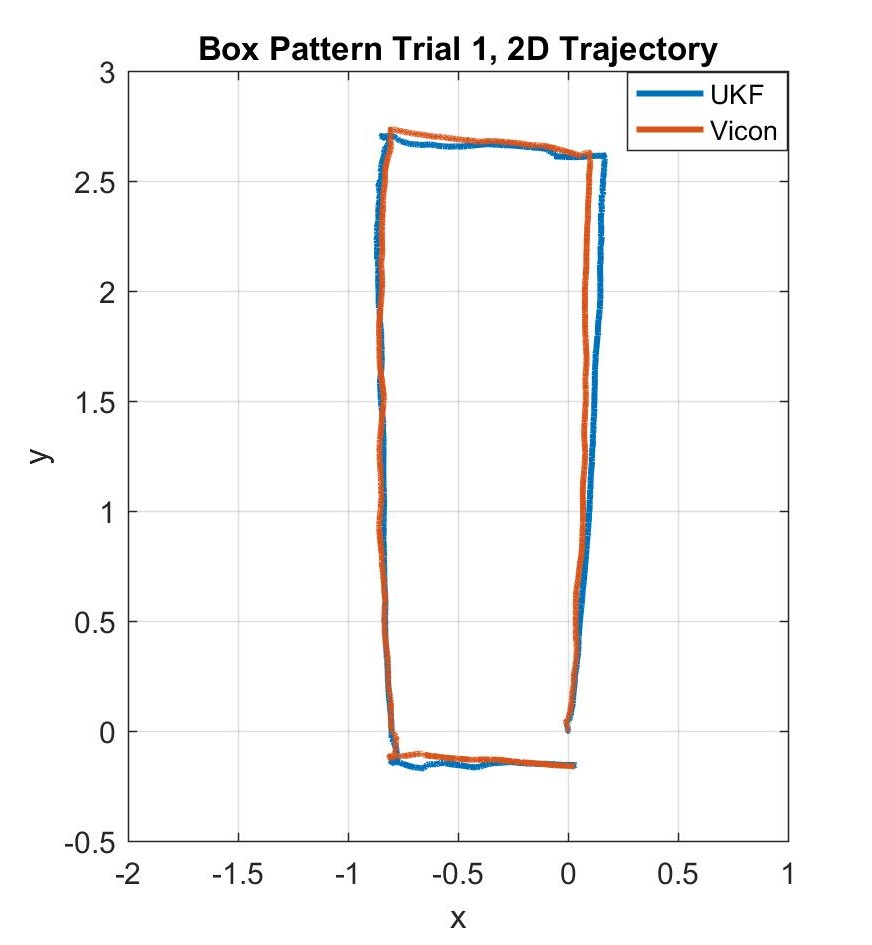
\includegraphics[width=\textwidth,left]{box1_2d}
    \end{subfigure}%
    ~ 
    \begin{subfigure}{0.6\textwidth}
        \centering
        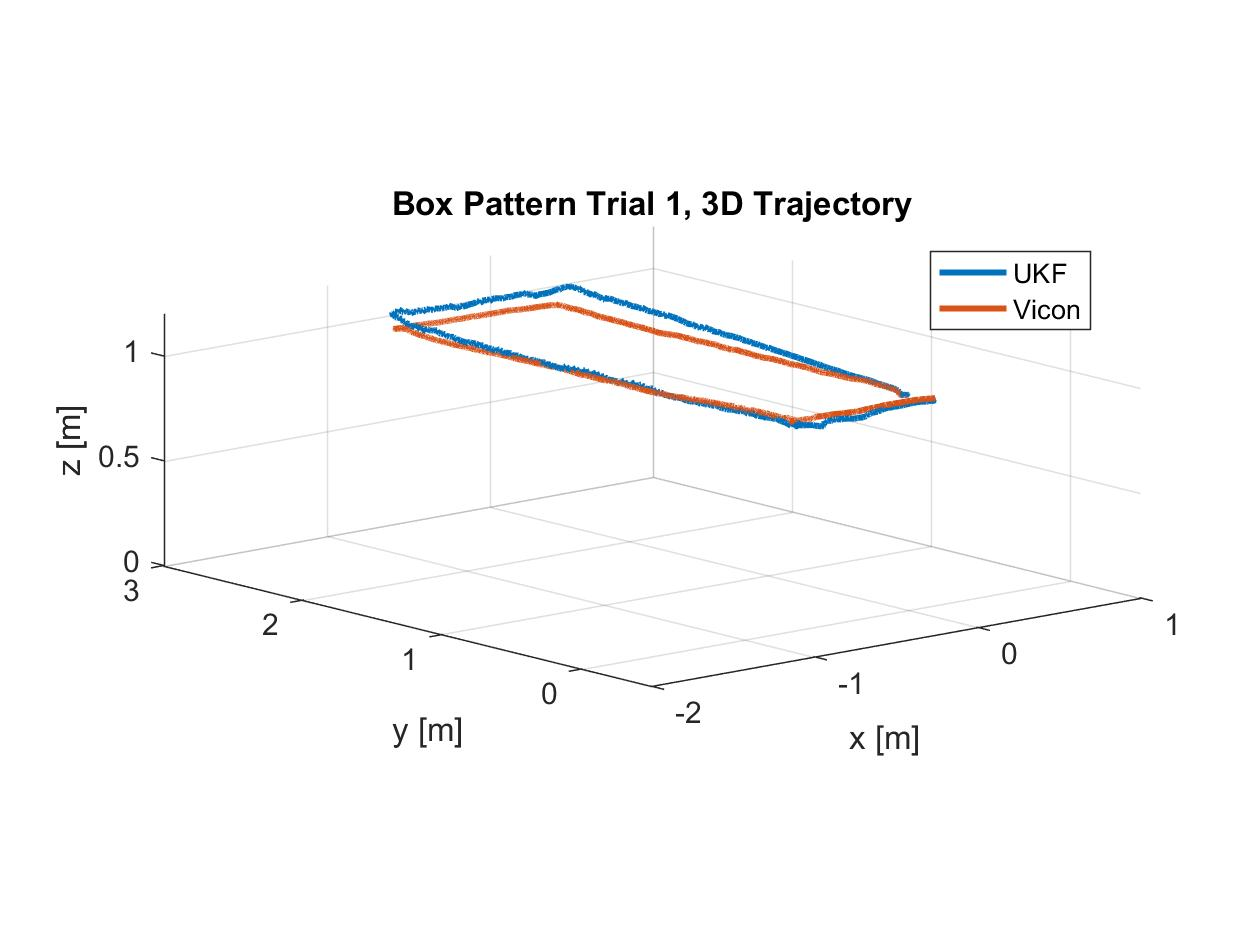
\includegraphics[width=\textwidth,right]{box1_3d}
    \end{subfigure}
    \caption[Box Pattern Trial 1 Trajectory]{2D and 3D trajectory plots from Box Pattern Trial~1.}
    \label{fig:box1_traj}
\end{figure}

\begin{figure}
    \centering
    \begin{subfigure}{0.4\textwidth}
        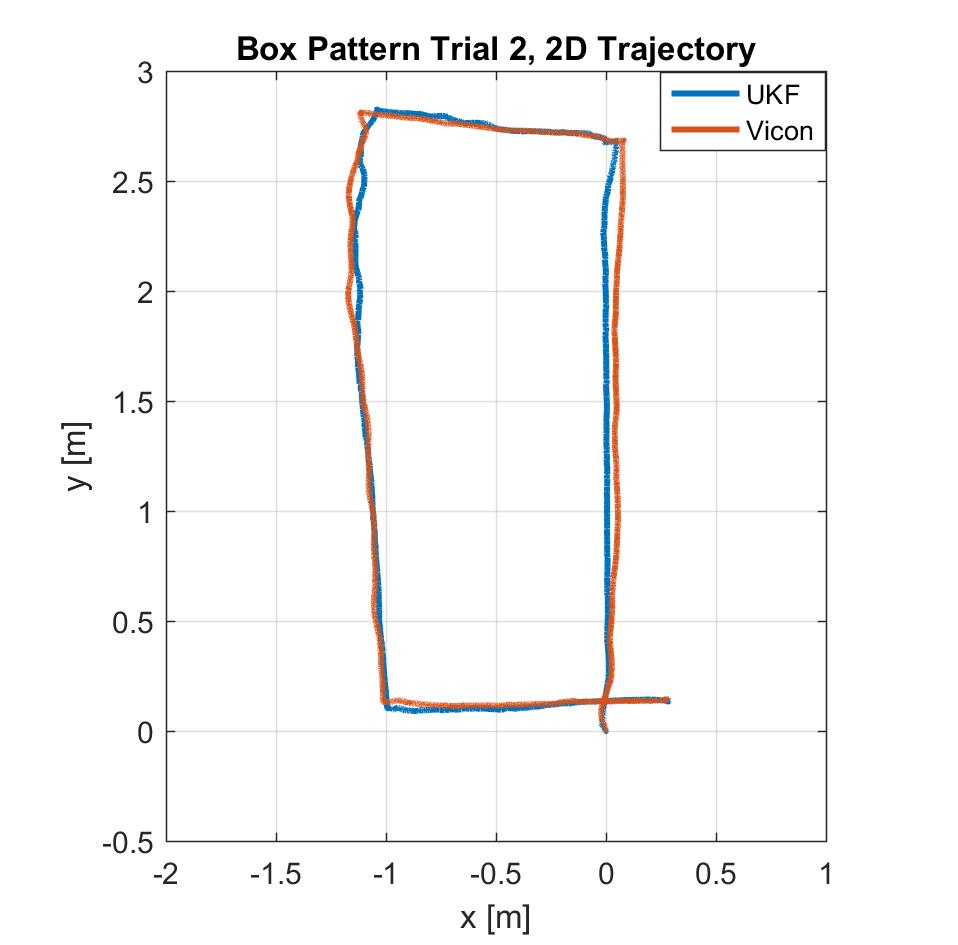
\includegraphics[width=\textwidth,left]{box2_2d}
    \end{subfigure}%
    ~ 
    \begin{subfigure}{0.6\textwidth}
        \centering
        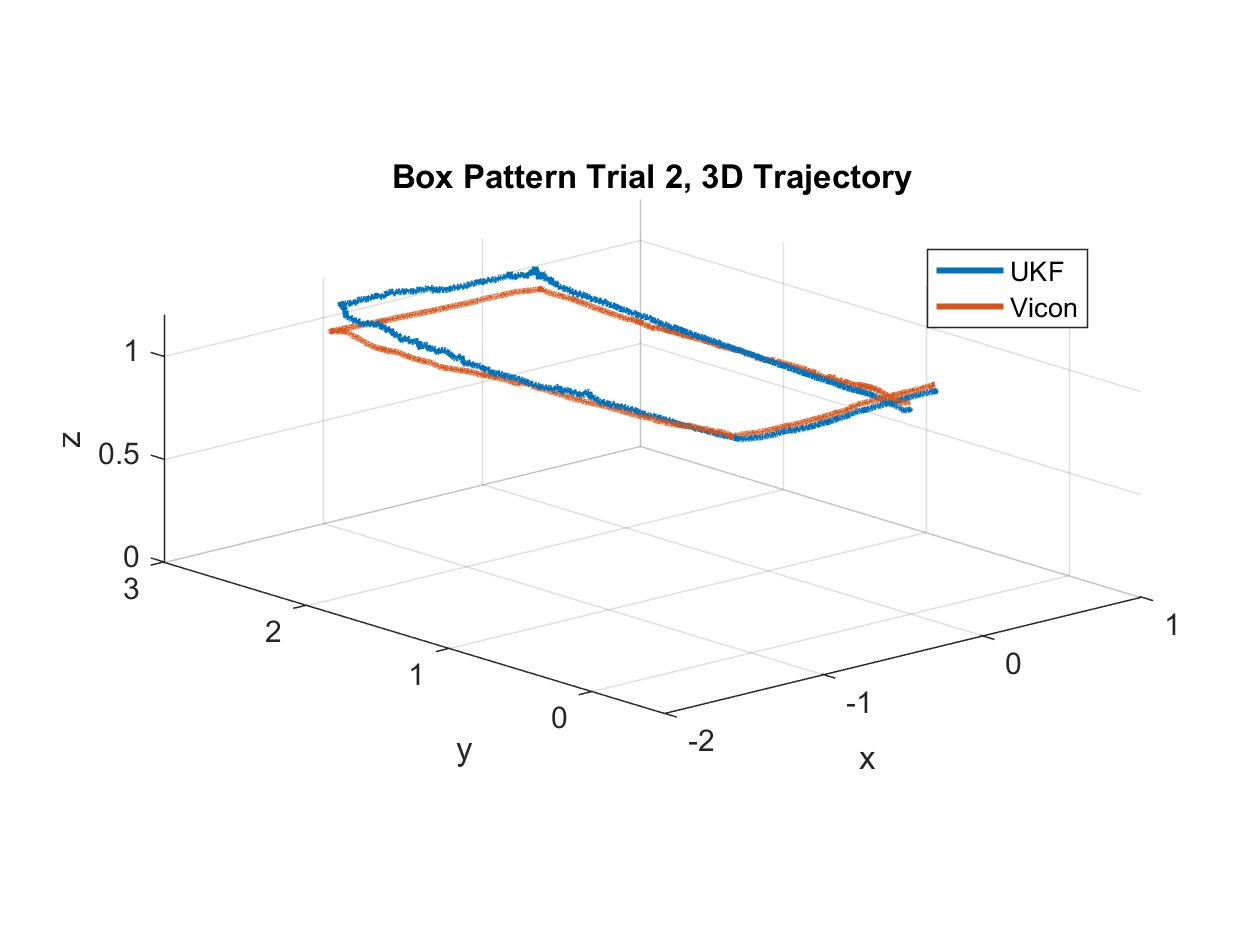
\includegraphics[width=\textwidth,right]{box2_3d}
    \end{subfigure}
    \caption[Box Pattern Trial 2 Trajectory]{2D and 3D trajectory plots from Box Pattern Trial~2.}
    \label{fig:box2_traj}
\end{figure}

\begin{figure}
    \centering
    \begin{subfigure}{0.4\textwidth}
        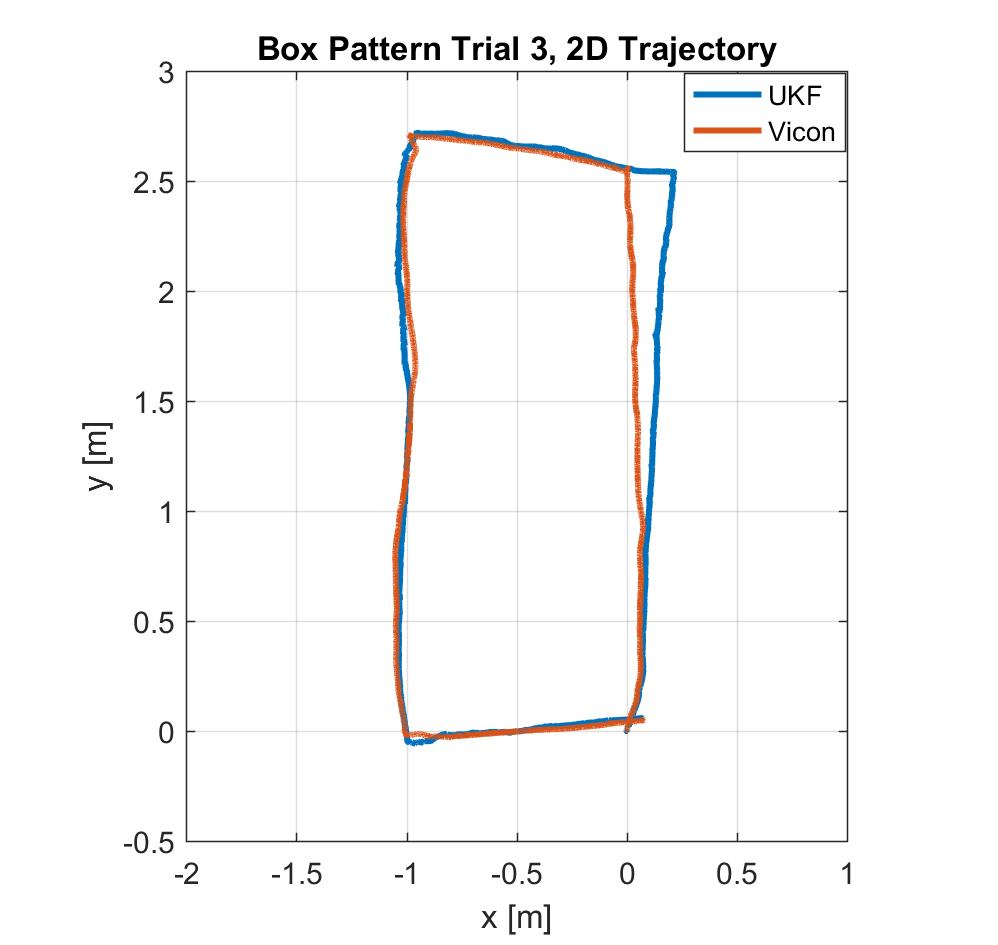
\includegraphics[width=\textwidth,left]{box3_2d}
    \end{subfigure}%
    ~ 
    \begin{subfigure}{0.6\textwidth}
        \centering
        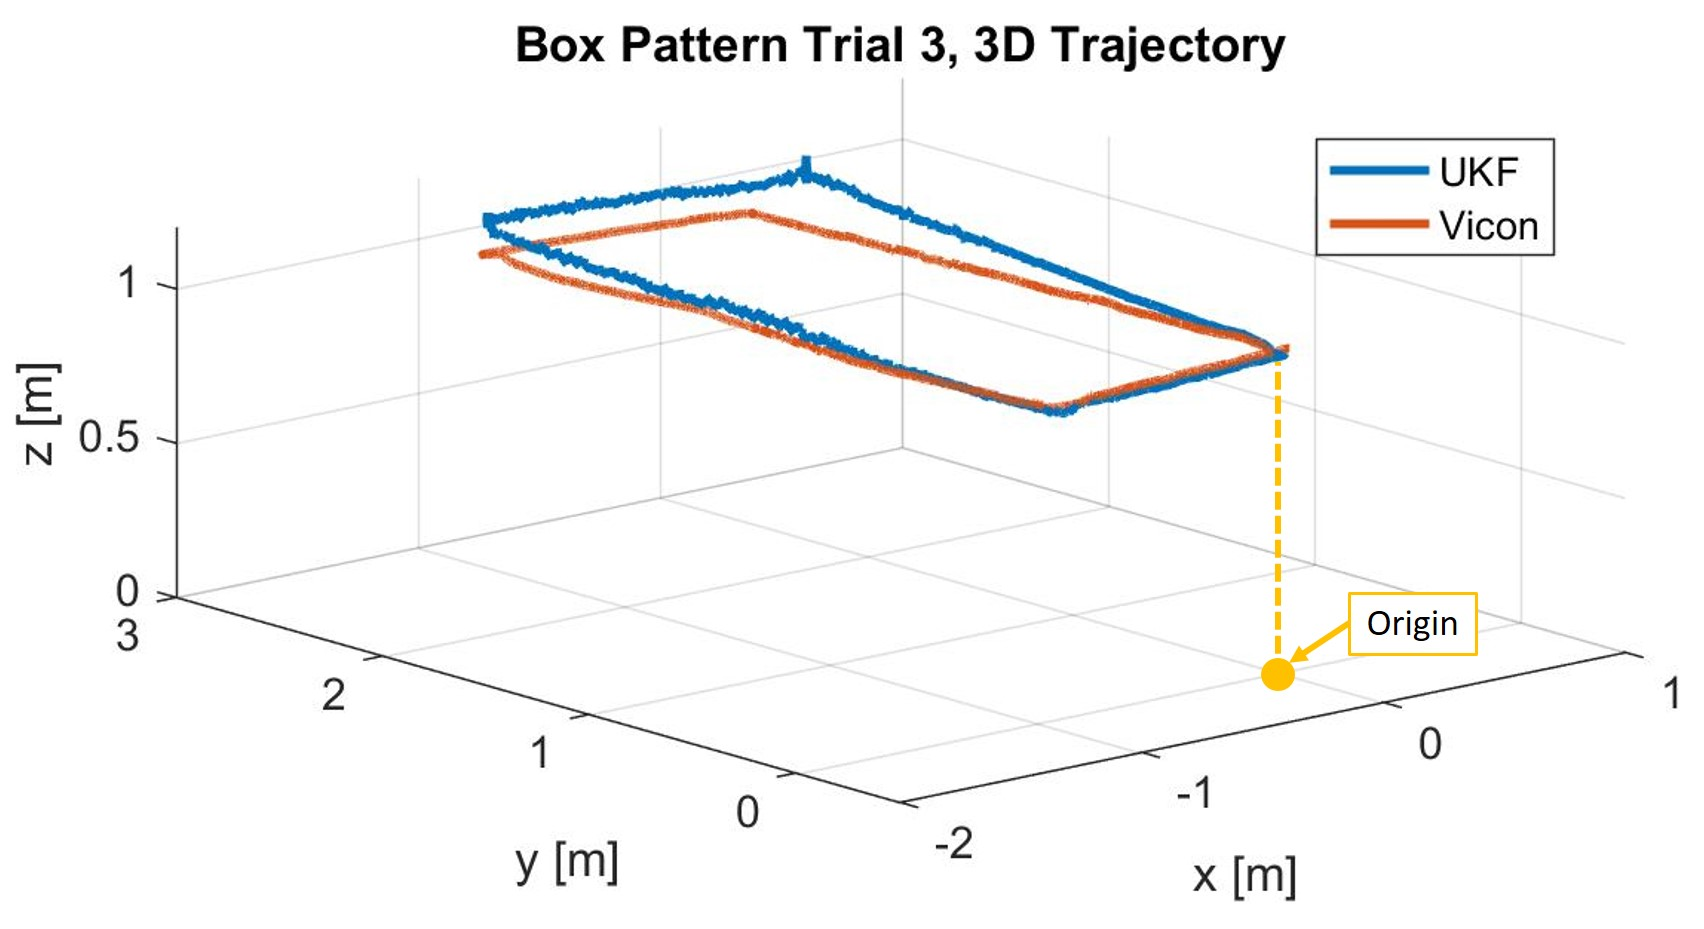
\includegraphics[width=\textwidth,right]{box3_3d}
    \end{subfigure}
    \caption[Box Pattern Trial 3 Trajectory]{2D and 3D trajectory plots from Box Pattern Trial~3.}
    \label{fig:box3_traj}
\end{figure}

\begin{figure}
    \centering
    \begin{subfigure}{0.4\textwidth}
        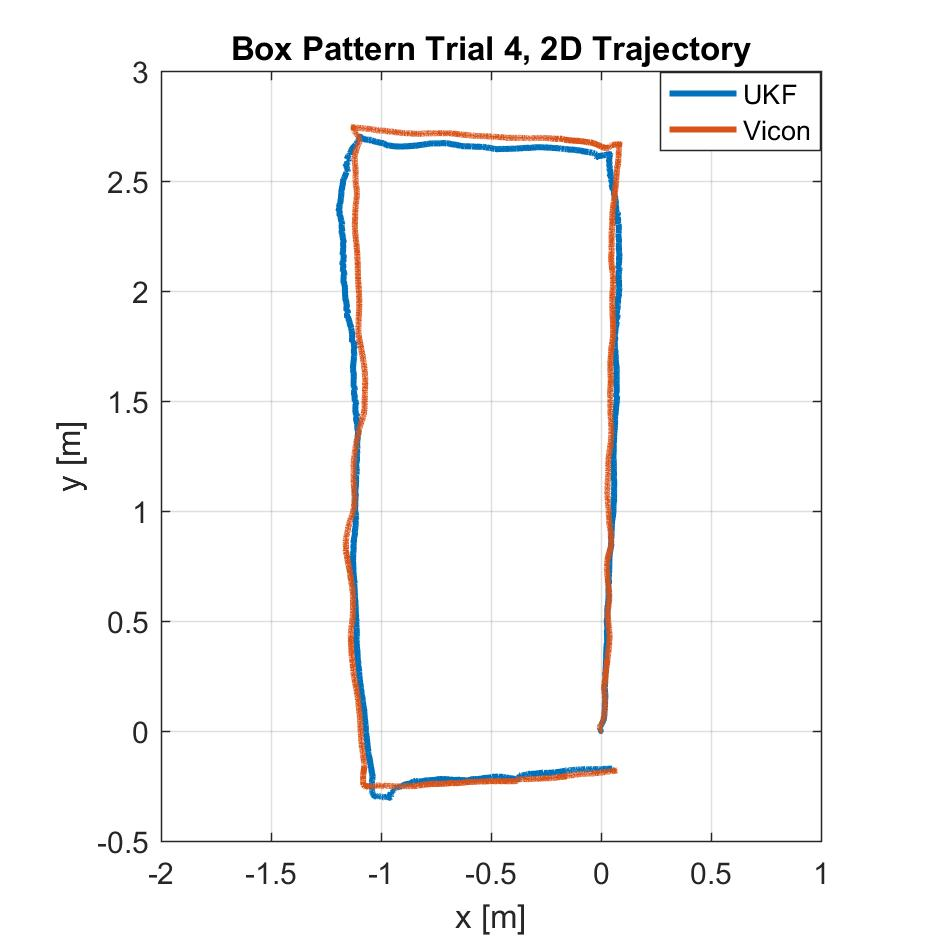
\includegraphics[width=\textwidth,left]{box4_2d}
    \end{subfigure}%
    ~ 
    \begin{subfigure}{0.6\textwidth}
        \centering
        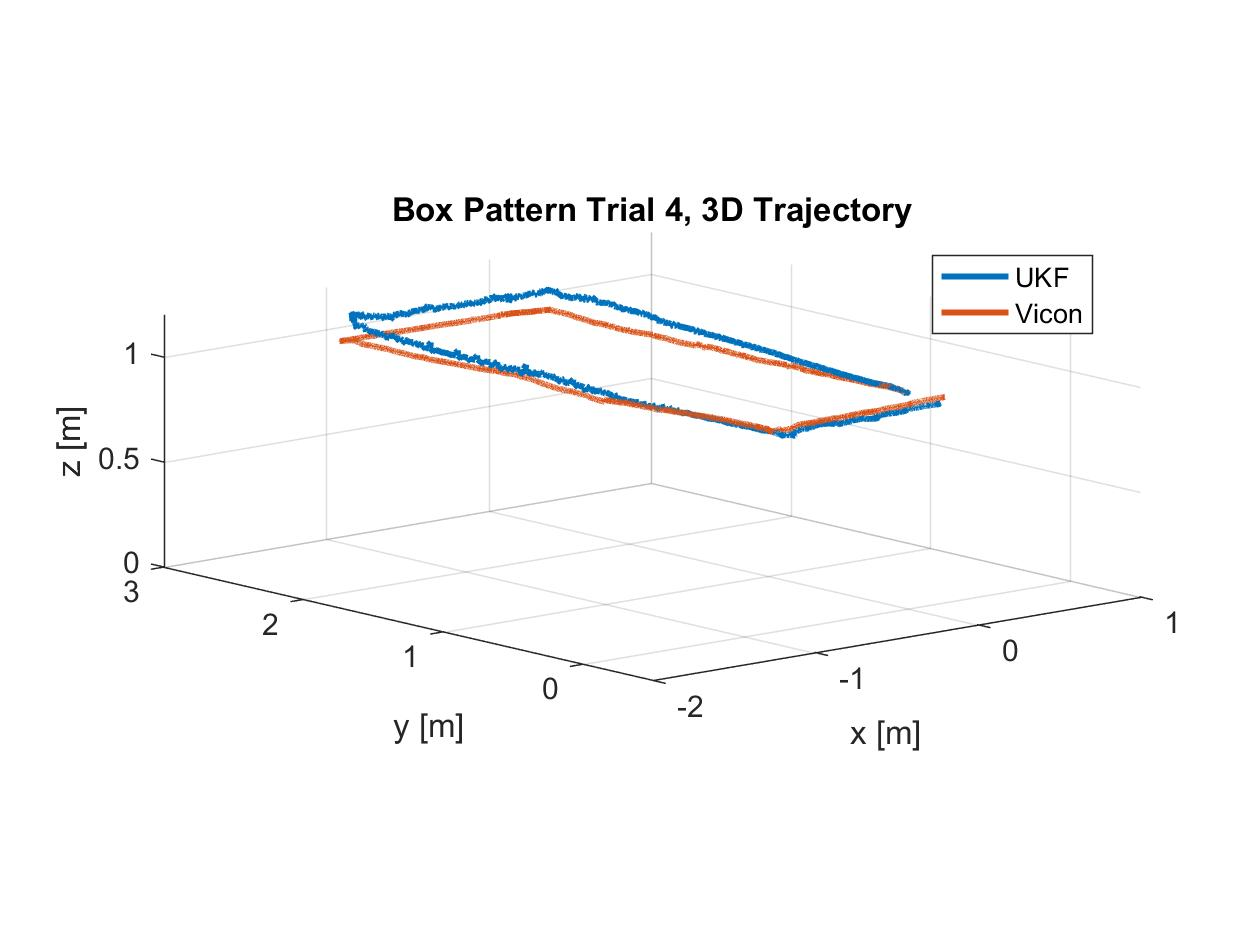
\includegraphics[width=\textwidth,right]{box4_3d}
    \end{subfigure}
    \caption[Box Pattern Trial 4 Trajectory]{2D and 3D trajectory plots from Box Pattern Trial~4.}
    \label{fig:box4_traj}
\end{figure}

\begin{figure}
    \centering
    \begin{subfigure}{0.4\textwidth}
        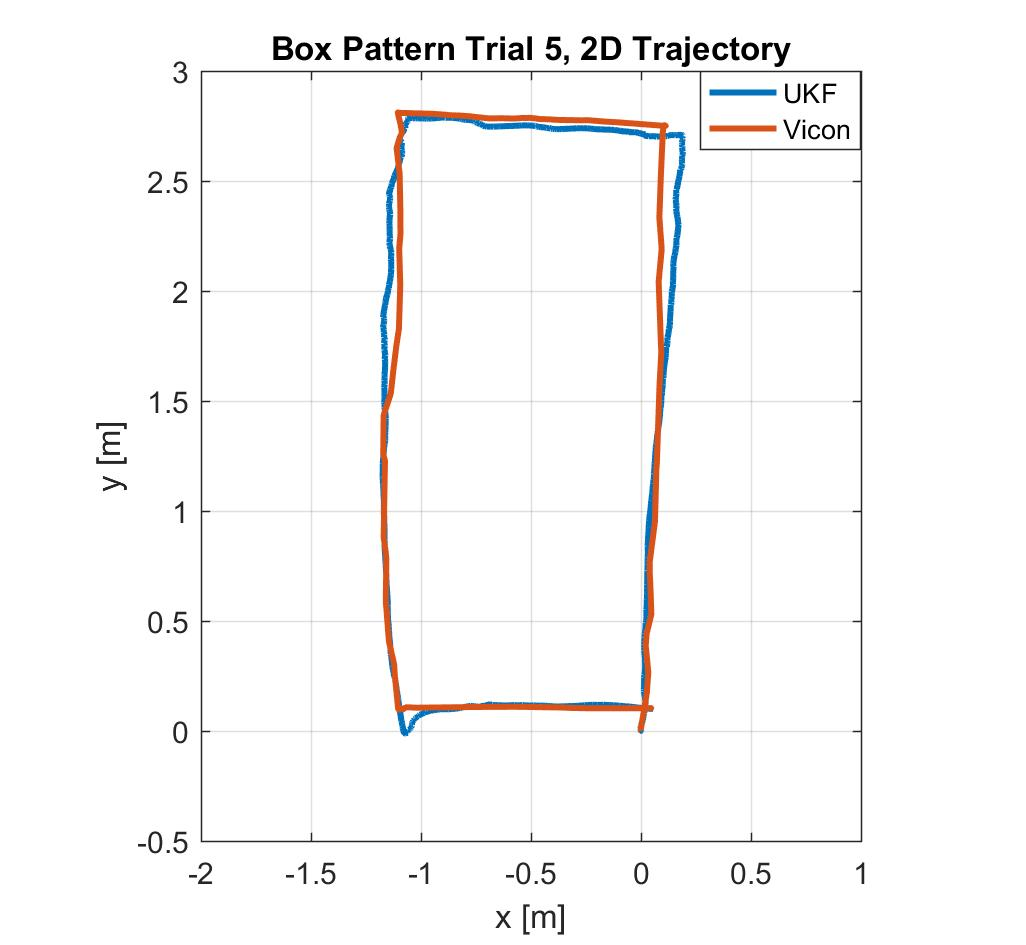
\includegraphics[width=\textwidth,left]{box5_2d}
    \end{subfigure}%
    ~ 
    \begin{subfigure}{0.6\textwidth}
        \centering
        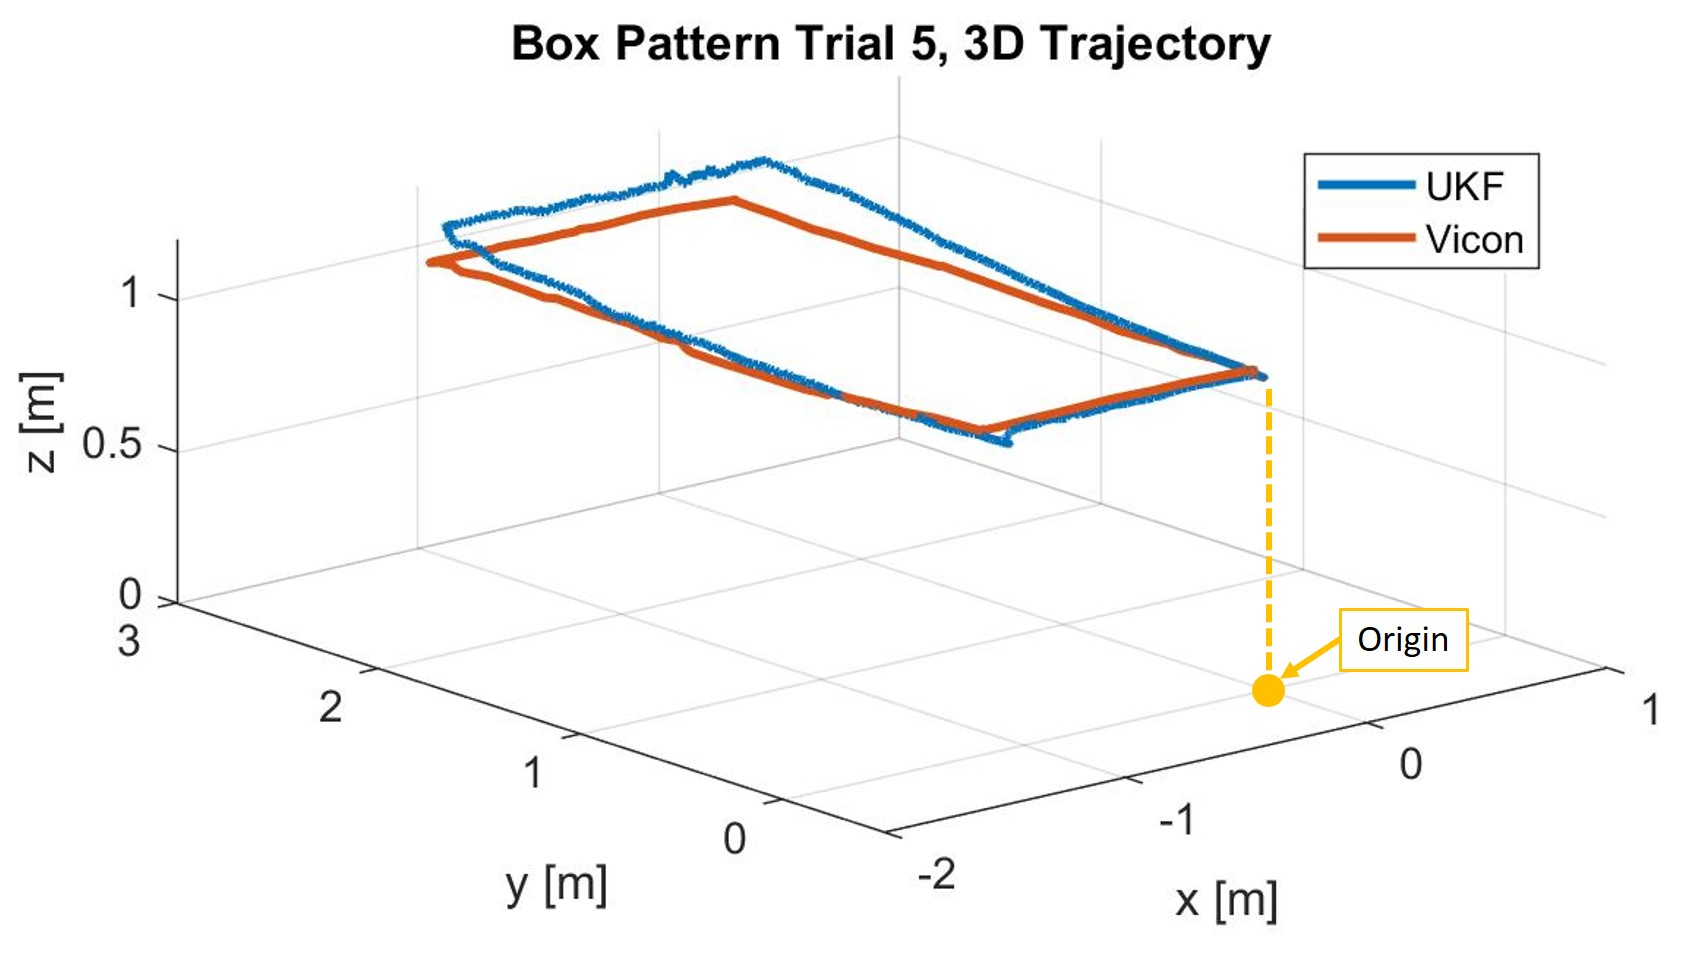
\includegraphics[width=\textwidth,right]{box5_3d}
    \end{subfigure}
    \caption[Box Pattern Trial 5 Trajectory]{2D and 3D trajectory plots from Box Pattern Trial~5.}
    \label{fig:box5_traj}
\end{figure}

\begin{figure}
  \centering
    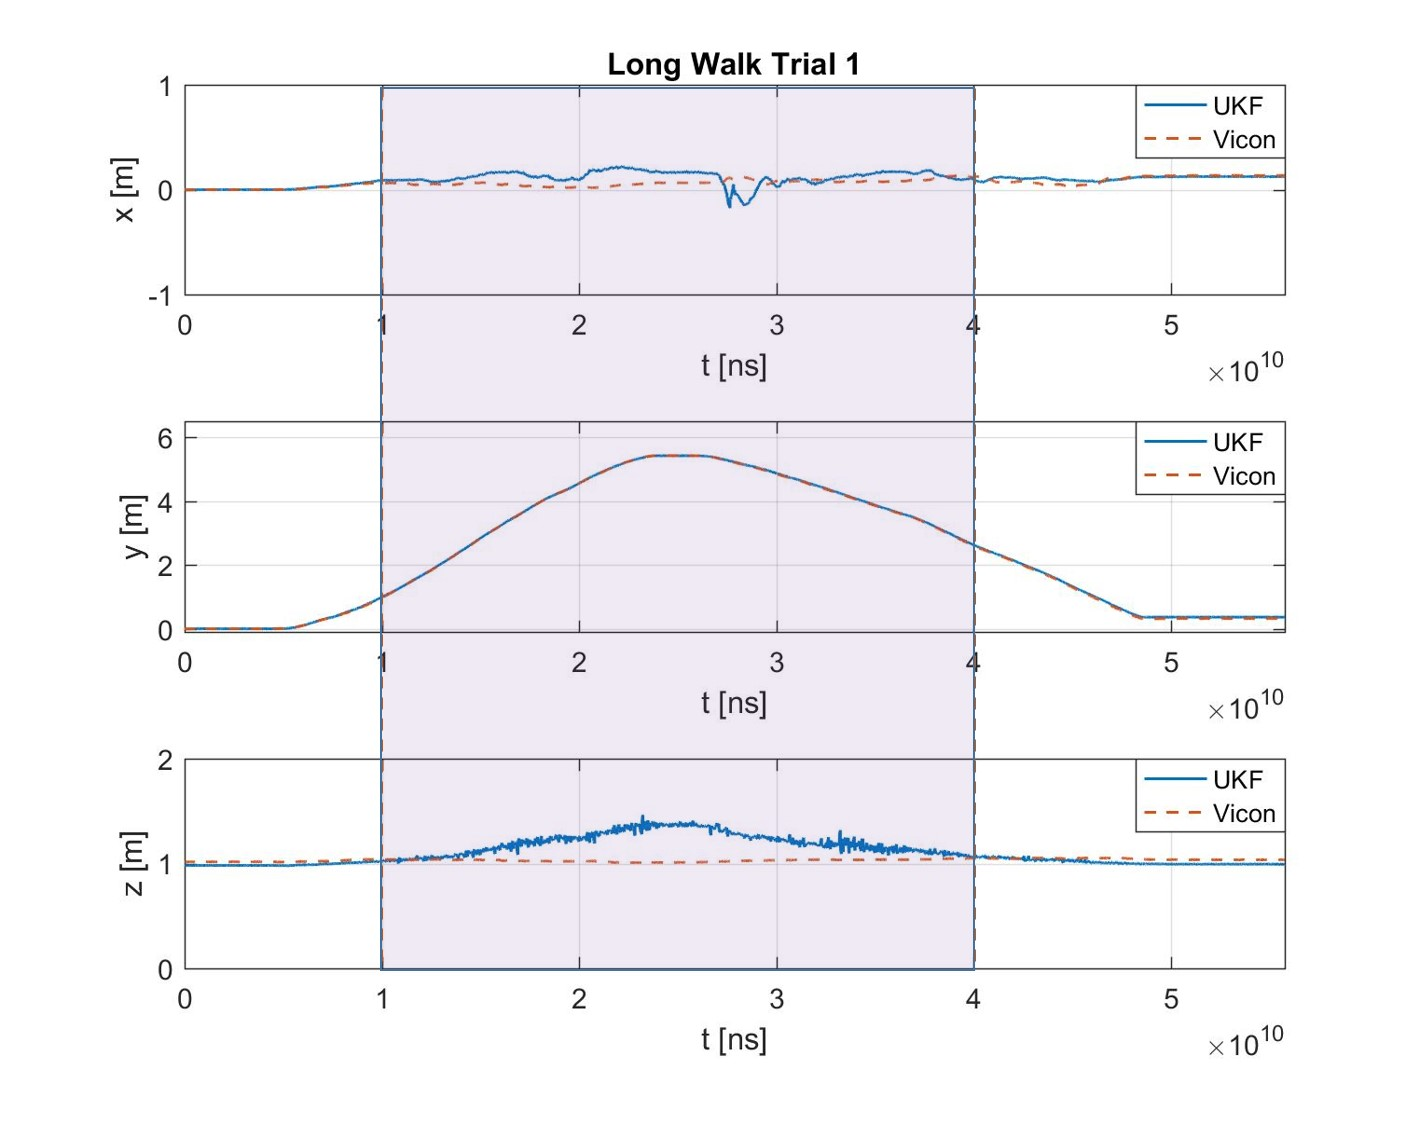
\includegraphics[width=\textwidth]{longWalk1_xyz}
  \caption[Long Walk Trial 1]{Long Walk Trial 1 coordinate plots. The shaded region highlights aberrant behavior coinciding with maximal displacement from the origin.}
  \label{fig:longWalk1_xyz}
\end{figure}

\begin{figure}
  \centering
    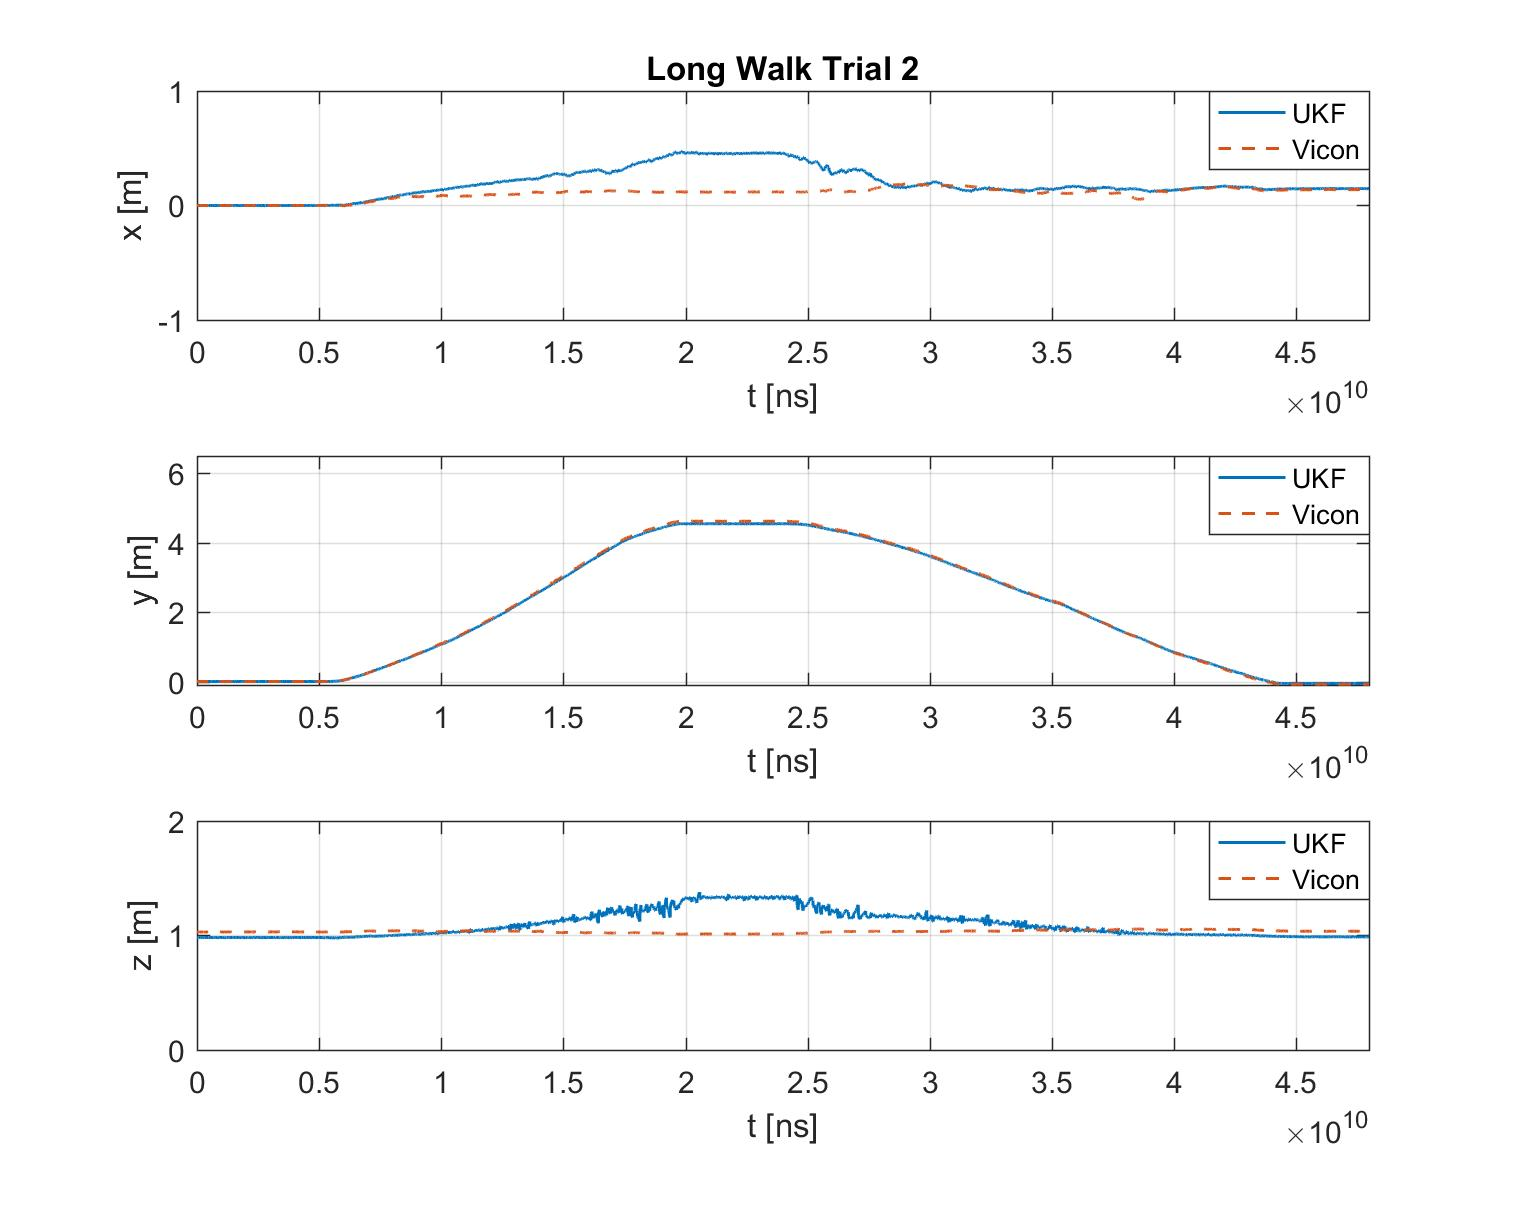
\includegraphics[width=\textwidth]{longWalk2_xyz}
  \caption[Long Walk Trial 2]{Long Walk Trial 2 coordinate plots.}
  \label{fig:longWalk2_xyz}
\end{figure}

\begin{figure}
  \centering
    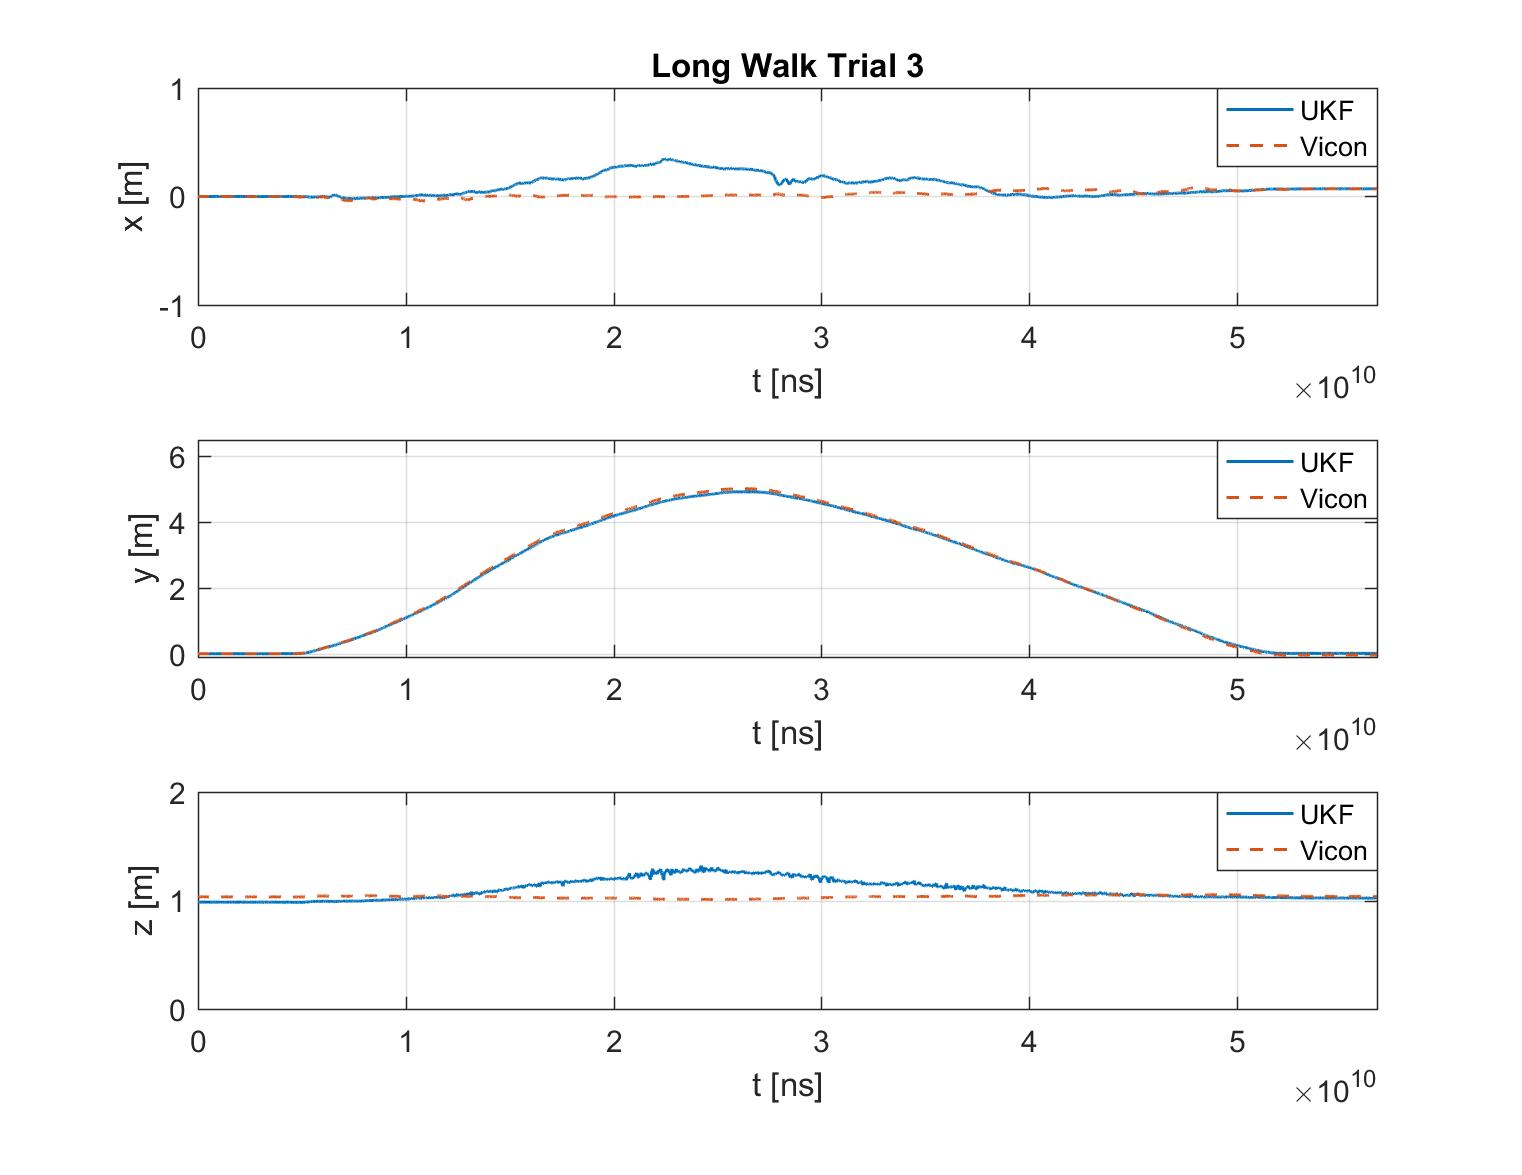
\includegraphics[width=\textwidth]{longWalk3_xyz}
  \caption[Long Walk Trial 3]{Long Walk Trial 3 coordinate plots.}
  \label{fig:longWalk3_xyz}
\end{figure}

\begin{figure}
  \centering
    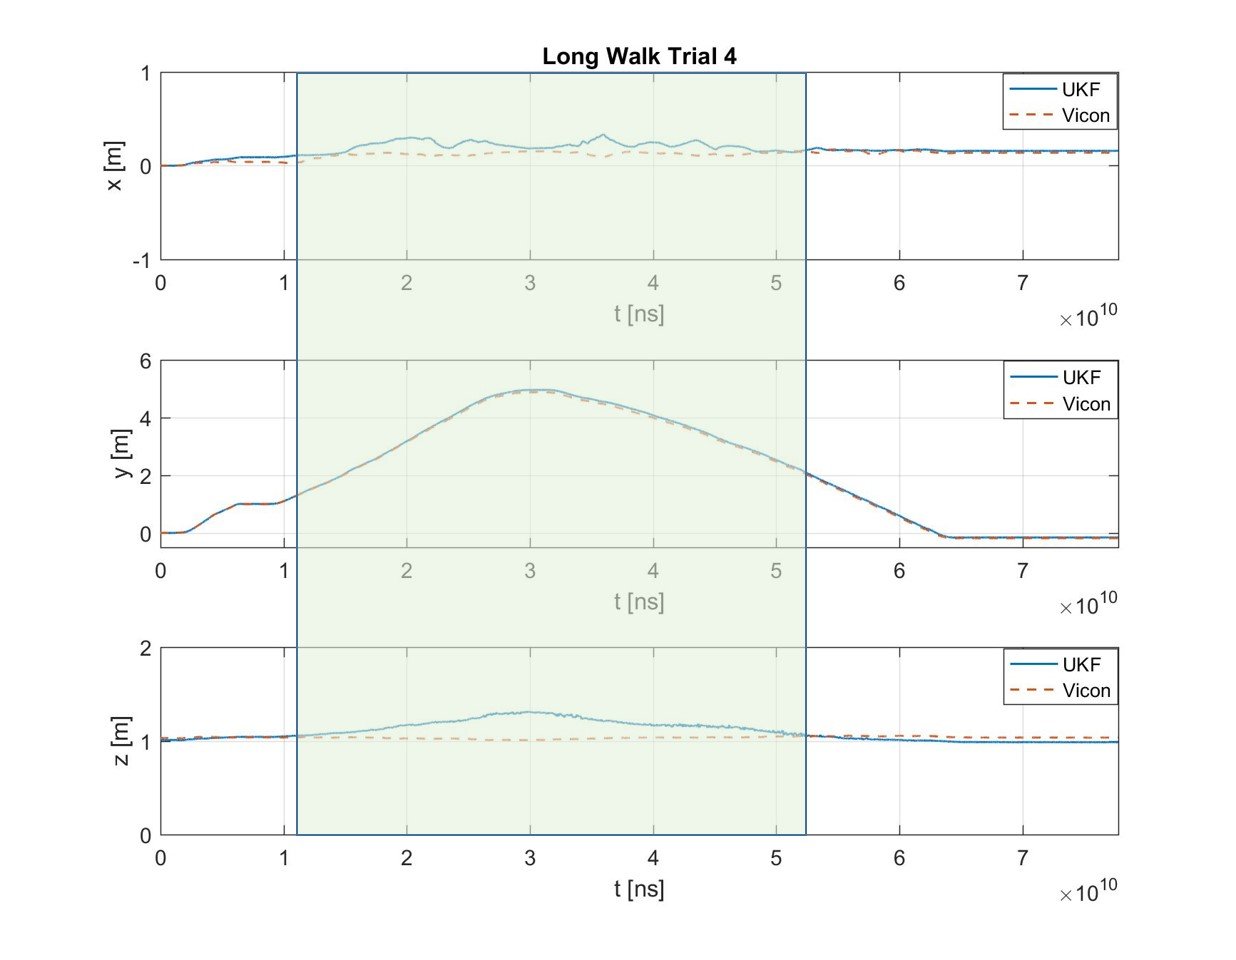
\includegraphics[width=\textwidth]{longWalk4_xyz}
  \caption[Long Walk Trial 4]{Long Walk Trial 4 coordinate plots.}
  \label{fig:longWalk4_xyz}
\end{figure}

\begin{figure}
  \centering
    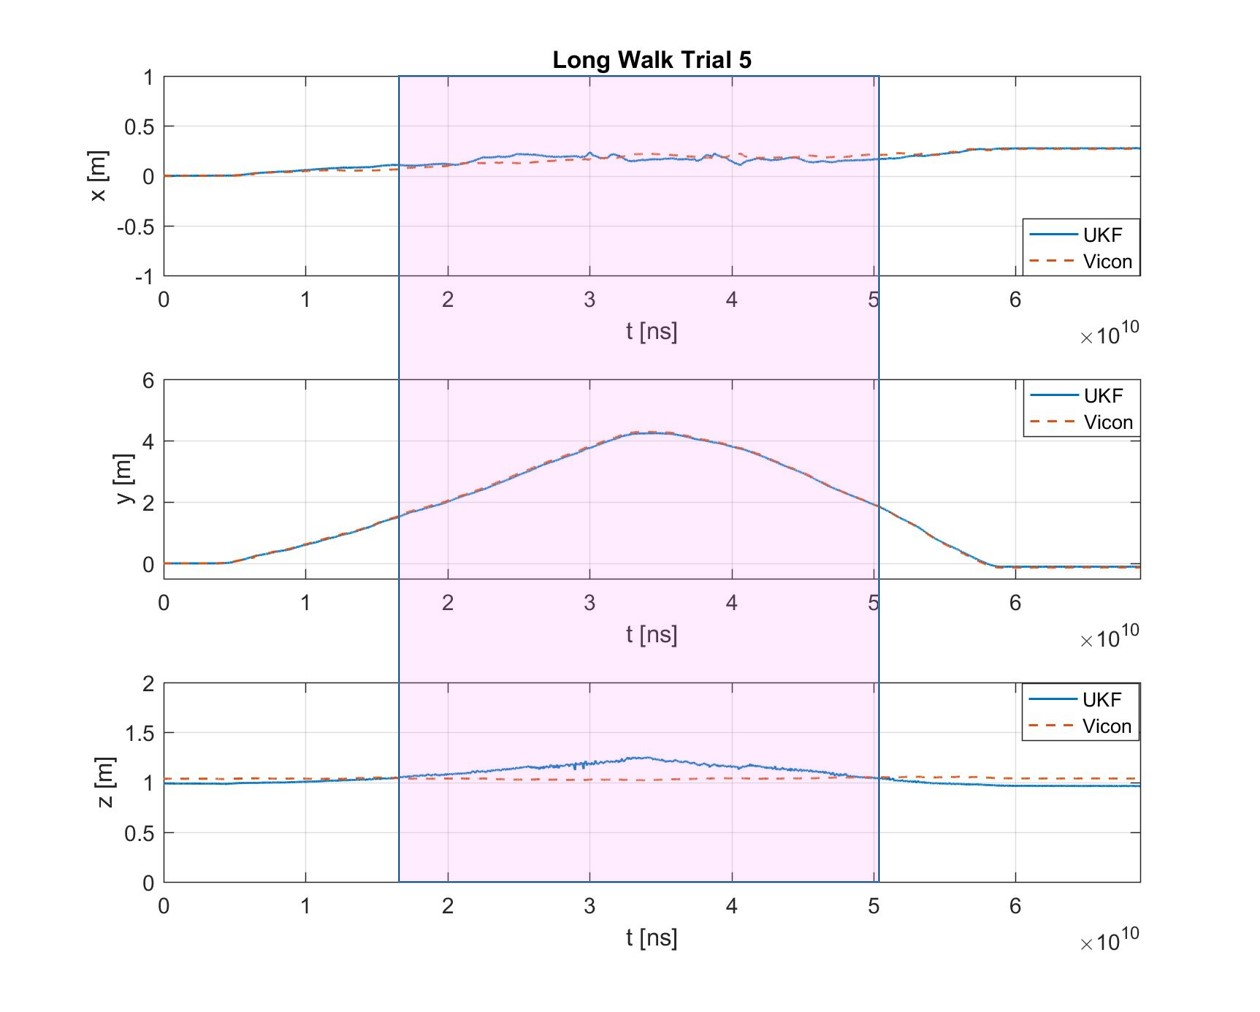
\includegraphics[width=\textwidth]{longWalk5_xyz}
  \caption[Long Walk Trial 5]{Long Walk Trial 5 coordinate plots.}
  \label{fig:longWalk5_xyz}
\end{figure}